\documentclass[12pt,xcolor=dvipsnames]{beamer}
\usetheme{CambridgeUS}
\usecolortheme{whale}
\setbeamercolor{block title}{use=structure,fg=white,bg=blue!75!black}  
\setbeamercolor{block body}{use=structure,fg=black,bg=blue!5!white}
\setbeamercolor{frametitle}{bg=Blue}

\usepackage{hyperref}   
\usepackage{url}
\hypersetup{urlcolor=red}

\renewcommand{\bibname}{References}
\setbeamertemplate{bibliography item}{[\theenumiv]}

\usepackage{multicol}
\usepackage{verbatim} 
\usepackage{graphics}
\usepackage{graphicx}


%Basic Information
\title{Motivation of the edX InSight Project}
\author{Arinjoy Basak et al.}
\date{\today}

%--------------------------------------------------------------------------------------
%               TITLE PAGE (Slide 1)
%--------------------------------------------------------------------------------------
\begin{document}
\begin{frame}
\titlepage
\end{frame}
%--------------------------------------------------------------------------------------


%--------------------------------------------------------------------------------------
%               Outline
%--------------------------------------------------------------------------------------
%\begin{frame}
%\frametitle{Outline}
%\begin{multicols}{2}
%\tableofcontents[hideallsubsections]
%\end{multicols}
%\end{frame}

%--------------------------------------------------------------------------------------
%               Slide 1: Topic 1
%--------------------------------------------------------------------------------------
\section{What our project is on}
\begin{frame}[t]
\frametitle{What is edX InSight?}

\begin{itemize}
\item InSight is a BI (Business Intelligence) platform that was built by edX for the purpose of communicating
the details of the courses, and analytical data concerning the student activity on the various courses to
the administrators and course instructors.\\

\item The primary aim of this platform is not only to monitor the
student performances and validation of the choices made in designing the course, but also allows the
designers to re-think the choices, and improve the course in its different aspects for creating a better
experience for the students.
\end{itemize}


%For bulleted points use the following:\\
%\begin{itemize}
% \item write point 1
% \item write poin 2
%\end{itemize}

%For numbered list use the following:\\
%\begin{enumerate}
% \item write point 1
% \item write point 2
%\end{enumerate}

\end{frame}
%--------------------------------------------------------------------------------------
%               Slide 2
%--------------------------------------------------------------------------------------
\section{What our project is on}
\begin{frame}[t]
\frametitle{What is edX InSight?}

\begin{itemize}

\item Insight is essentially a Django application that allows instructors and administrators to know about
their students with respect to.

\begin{itemize}
\item course activity
\item demographic distributions
\item location based distributions, and 
\item educational qualifications
\end{itemize}

\item The unstructured data in the form of events
are stored in Amazon S3 as JSON objects, while the processed data is then stored in MySQL. Insight
uses MySQL 5.1 for its purpose. The data is then transferred to Insights via a REST API.

\end{itemize}
\end{frame}

%--------------------------------------------------------------------------------------
%               Slide 3
%--------------------------------------------------------------------------------------
\section{What our project is on}
\begin{frame}[t]
\frametitle{What our project is}

\begin{itemize}

\item Our main project tasks are to study the edX InSight system and contribute towards its development and final integration
with the IITBombayX MOOC Platform.

\item In particular, our aim will be to extend and implement the edX InSight services so that it appropriately suits to the 
Indian education environment.

\end{itemize}
\end{frame}


%--------------------------------------------------------------------------------------
%               Slide 4
%--------------------------------------------------------------------------------------
\section{Motivation of the edX InSight Project}
\begin{frame}[t]
\frametitle{Why do we need InSight?}

\begin{itemize}
\item The study by Ma, Han, Yang and Chen analysed the the impact of an instructor on a student’s engagement in an online learning environment, by building an interaction activity model for the teaching and learning process.

\item It was showed that learning data analytics could be used
to capture authentic, timely and objective evidence regarding online learning behaviour, with a focus
towards college level online learning environments.

\item The course was the unit of analysis, not the student.

\end{itemize}
\end{frame}
%--------------------------------------------------------------------------------------
%               Slide 5
%--------------------------------------------------------------------------------------
\section{Motivation of the edX InSight Project}
\begin{frame}[t]
\frametitle{Why do we need InSight?}

edX Insight provides access to various graphs, metrics and reports for analysing the student be-
haviour and activity in different aspects, such as :

\begin{itemize}

\item Course Enrollment data : daily student enrollment chart, enrollment metric, and enrollment over time metrics.

\item Engagement Data : weekly engagement charts, content engagement breakdown report.
\item Demographic Data : analytics on age bands and educational backgrounds.
\item Location/Geographic Data : enrollment geography.
\item Data on graded and ungraded contents : Find points of difficulty, and attempts to solve the problems.

\end{itemize}
\end{frame}

%--------------------------------------------------------------------------------------
%               Slide 6
%--------------------------------------------------------------------------------------
\section{Motivation of the edX InSight Project}
\begin{frame}[t]
\frametitle{}

\begin{itemize}
\item 
\end{itemize}
\end{frame}

%--------------------------------------------------------------------------------------
%               Slide 7
%--------------------------------------------------------------------------------------
\section{Motivation of the edX InSight Project}
\begin{frame}[t]
\frametitle{Project application Idea 1}

\begin{itemize}
\item Analyse the student learning behaviour and activities through the pauses in the lecture videos.
\item The locations of the pauses could be collected as events, and metrics could be developed and appropraite visualizations made to notify or warn the instructors about the difficulty faced by students in particular parts of materials.
\item This could then be met by appropriate measures on the teacher's end, such as

\begin{itemize}
\item Adding more explanatory material
\item Release of an expansion video
\item More quizzes ad practice exercises.
\end{itemize}

\end{itemize}
\end{frame}

%--------------------------------------------------------------------------------------
%               Slide 8
%--------------------------------------------------------------------------------------
\section{Motivation of the edX InSight Project}
\begin{frame}[t]
\frametitle{Project application idea 1}
\hfill
\hfill
\begin{itemize}
\item API exists for such tracking, and we can have a possible flow such as the following:
\hfill
\begin{center}
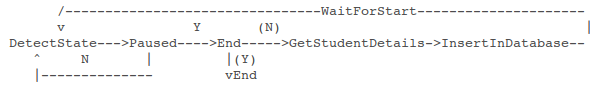
\includegraphics[height=1.8cm]{Diag1.png}\\ % Insert your image it this way
\end{center}

\end{itemize}

\end{frame}

%--------------------------------------------------------------------------------------
%               Slide 9
%--------------------------------------------------------------------------------------
\section{Motivation of the edX InSight Project}
\begin{frame}[t]
\frametitle{Project application idea 2}

\begin{itemize}
\item Create dashboard system for students based on their own course activity and performance
\item Allow the students to understand whether they are either falling behind the others on their progress, at par with the other students, or ahead of the other students in learning
\item This could be implemented as a mobile application too, refreshed with the analysed data and visualizations after a certain time period.
%\item Inspired by Erik Duval's speech at TEDxUHowest
\end{itemize}
\end{frame}

%--------------------------------------------------------------------------------------
%               Slide 10
%--------------------------------------------------------------------------------------
\section{Motivation of the edX InSight Project}
\begin{frame}[t]
\frametitle{Project application idea 3}

\begin{itemize}
\item The communication and interaction between the students could be collected
\hfill
\item We can then use this data to visualize the communication and interaction between the students, to find he students/student groups who are in close communication, and those who aren't in close communication and are slightly outside this conglomerate, residing on the edges.
%\item Inspired by Erik Duval's speech at TEDxUHowest
\end{itemize}
\end{frame}

%--------------------------------------------------------------------------------------
%               Slide 11
%--------------------------------------------------------------------------------------
\section{Motivation of the edX InSight Project}
\begin{frame}[t]
\frametitle{Project application idea 4}

\begin{itemize}
\item A spectral band image system for determining the student's performance
\item ---) Because people understand images better than text or data! (:D)
\item The spectrum would have different colours for different areas (examinations, lessons, mood of students, activity overall)
\item Intensity of the colours depicts performance.
\item The degree of transitions between the individual regions determines the balance of the activities.

\end{itemize}
\end{frame}

%--------------------------------------------------------------------------------------
%               Slide 12
%--------------------------------------------------------------------------------------
\section{Motivation of the edX InSight Project}
\begin{frame}[t]
\frametitle{Project application idea 5}

\begin{itemize}
\item For each pair of students chosen at a time, show a graphical measure to determine interaction among any two students chosen at a time.
\item For example, a colour spectrum with the degree of transition showing the amount of interaction between the students (may even extend to student and teacher/instructor)
\item Can be used for determining homogeneity in student population and points of disturbances (less interaction, ineffective activity, behind others in progress, and so on).

\end{itemize}
\end{frame}


%--------------------------------------------------------------------------------------
%               Slide 3: Topic 2
%--------------------------------------------------------------------------------------
\section{Topic 2}
\begin{frame}[t]
\frametitle{Topic 2}
Use the following for creating a table \\
\begin{center}
\begin{tabular}{|c|c|c|}
 \hline
 No. & Name & Project \\
 \hline
 1 & Firuza & Code::Blocks \\
 \hline
 2 & Birundha & edX \\
 \hline
\end{tabular}
\end{center}
\end{frame}


%---------------------------------------------------------------------------------------
%     Final Slide - References
%--------------------------------------------------------------------------------------
\section{References}
\frametitle{References}
\begin{frame}[allowframebreaks]{References}
\bibliographystyle{ieeetr}
\bibliography{biblio}
\end{frame}
\end{document}
